

\section{K-means Clustering in R}

The \texttt{kmeans()} function calculates standard k-means clusters in R.  The input is a data matrix (perhaps transformed before hand) and $k$, the number of clusters. Alternatively you can specify starting cluster centers. You can also run the algorithm multiple times with different random starting positions by using the \texttt{nstart} argument.

\begin{R}
# generate data set w/two groups (one of size 50, the other of size 75)
# note the different means and std dev between the two groups
> test.data <- rbind(matrix(rnorm(100, mean=0, sd=0.2),ncol=2), 
                  matrix(rnorm(150,mean=1,sd=0.5),ncol=2))
> colnames(test.data) <- c("x", "y")
> plot(test.data)
> cl <- kmeans(test.data, 2)
> names(cl)
[1] "cluster"  "centers"  "withinss" "size"    
> cl$cluster #  which cluster each object is assigned to
... output deleted ...
> plot(test.data, col = cl$cluster)
> cl$centers  # compare to the "true" means for the groups
            x         y
1 0.009479636 0.1182016
2 1.109641398 1.0427396
> points(cl$centers, col = 1:2, pch = 8, cex=2)

> # what if we pick the wrong number of clusters?
> cl <- kmeans(test.data, 5)
> plot(test.data, col = cl$cluster)
> points(cl$centers, col = 1:5, pch = 8, cex=2)

> # as above but using nstart argument
> cl <- kmeans(test.data, 5, nstart=25)
> plot(test.data, col = cl$cluster)
> points(cl$centers, col = 1:5, pch = 8, cex=2)
\end{R}

\subsection{Applying K-means to the iris data set}

Now that we've seen how to apply k-mean clustering to a synthetic data set, let's go ahead and apply it to our old friend, the iris data set. Note that this is a four dimensional data set so we'll need to pick a projection in which to depict the cluster.  The space of the first two principal components is a natural choice (but note that the fact that we're using the PCA space doesn't impact the k-means clustering in this context).

\begin{R}
# drop the fifth column (species names)
# we'll assume we know how many groups there are    
> k.iris <- kmeans(as.matrix(iris[,-5]), 3)    
> iris.pca <- prcomp(iris[,-5])
# the following plot colors the specimens by the group
# they were assigned to by the k-means clustering
> plot(iris.pca$x,col=k.iris$cluster)

# this plot colors specimens by k-means grouping
# and chooses plot symbol by real species grouping.
# This can help us quickly pick out the misclasssified
# specimens
> plot(iris.pca$x, col=k.iris$cluster, pch=c(1,2,16)[iris[,5]])
\end{R}


\section{K-means clustering in Python}

The module |scipy.cluster.vq| in the SciPy package implements k-means clustering.  Using this module, there are three key steps you need to carry out: 1) normalizing (whitening) the input data set using the |whiten()| function; 2) running the |kmeans()| algorithm to calculate the cluster centroids; and 3) assigning each observation to the respective cluster using the |vq()| function (``vq'' is short for vector quantization).
%
\begin{python}
>>> irisDF = pd.read_csv('iris.csv')
>>> iris = irisDF[irisDF.columns[:4]].values
>>> from scipy.cluster import vq
>>> normiris = vq.whiten(iris)

# std deviation of variables before normalization
>>> np.std(iris,axis=0)
array([ 0.82530129,  0.43441097,  1.75940407,  0.75969263])

# std deviation of variables after normalization
>>> np.std(normiris,axis=0)
array([ 1.,  1.,  1.,  1.])

# calculate kmeans, using 3 groups
>>> centroids, distortion = vq.kmeans(normiris, 3)
>>> centroids
array([[ 7.00300835,  6.10726115,  2.45908867,  1.81598687],
       [ 8.14913325,  7.0954768 ,  3.10488375,  2.58102322],
       [ 6.06566359,  7.89114515,  0.83096318,  0.32381517]])

# Distortion is the sum of the squared diffs. btw. obs and corresponding centroids
>>> distortion
0.85998478065872275

# Assign each observation to it's nearest centroid
>>> assign, distortion = vq.vq(normiris, centroids)

# first ten items are assigned to group 2
>>> assign[:10]
array([2, 2, 2, 2, 2, 2, 2, 2, 2, 2])

# some more assignments
>>> assign[40:55]
array([2, 2, 2, 2, 2, 2, 2, 2, 2, 2, 1, 1, 1, 0, 0])
\end{python}

\subsection{Creating a PCA plot in Python}

Now that we've carried out the k-means clustering, let's generate a plot to illustrate the results.  As we did before, we'll project the specimens into the space of the first two principal components and then color the points using the centroid labels assigned by the k-means algorithm.  

As we saw in previous lectures, there is no built in PCA function in SciPy, but we can either implement one ourselves using the SVD functions, or we can make use of a prepackaged PCA function from one of the libraries like StatsModels or SciKit-Learn.  For today's exercises we'll make use of a PCA function in a library called MDP (`Modular toolkit for Data Processing', \url{http://mdp-toolkit.sourceforge.net/}).  

The MDP library isn't included by default in the Anaconda Python Distribution, so we'll have to install it. We'll do so using the |conda| command line tool that comes with Anaconda.  Make sure to enter the following commands in the shell (terminal/command prompt) \emph{not} from within the Python interpreter.

\begin{bash}
$ conda update conda  # updates the conda tool
$ conda update anaconda # updates already installed packages
$ conda install mdp
\end{bash}%$

Once the MDP library has been installed you can import it into your IPython session.

%
\begin{python}
>>> import mdp
>>> irispca = mdp.pca(iris)
# mdp.pca returns a matrix of PC scores.  The scores for each PC are in the columns
>>> irispca.shape
(150, 4)

# we'll draw each of the labeled groups separately
>>> group0 = irispca[assign == 0]
>>> group1 = irispca[assign == 1]
>>> group2 = irispca[assign == 2]
>>> plot(group0[:,0], group0[:,1], color='blue', marker='o', linestyle='none')
>>> plot(group1[:,0], group1[:,1], 'ro')  # shorthand way of plotting with red
                                          # circular markers; see help(plot) for info
>>> plot(group2[:,0], group2[:,1], 'go')
>>> axes = gca()  # get the python object that represents the plot axes
>>> axes.set_aspect('equal') # set equal aspect ratio for x- and y-axes
>>> draw()  # call draw() to refresh the plot
\end{python}

For the iris data set we know the true clustering.  The first 50 specimens are \textit{I.~setosa}, the next 50 \textit{I.~versicolor}, and the last 50 are \textit{I.~virginica}.  Let's create a fancier plot with with two subfigures. The left plot will be the k-means assignments again; the right plot will highlight the mis-assignments.
%
\begin{python}
# let's examine the centroid assignments
>>> assign
array([2, 2, 2, 2, 2, 2, 2, 2, 2, 2, 2, 2, 2, 2, 2, 2, 2, 2, 2, 2, 2, 2, 2,
       2, 2, 2, 2, 2, 2, 2, 2, 2, 2, 2, 2, 2, 2, 2, 2, 2, 2, 2, 2, 2, 2, 2,
       2, 2, 2, 2, 1, 1, 1, 0, 0, 0, 1, 0, 1, 0, 0, 0, 0, 0, 0, 1, 0, 0, 0,
       0, 1, 0, 0, 0, 0, 1, 1, 1, 0, 0, 0, 0, 0, 0, 0, 1, 1, 0, 0, 0, 0, 0,
       0, 0, 0, 0, 0, 0, 0, 0, 1, 0, 1, 1, 1, 1, 0, 1, 1, 1, 1, 1, 1, 0, 1,
       1, 1, 1, 1, 0, 1, 0, 1, 0, 1, 1, 0, 1, 1, 1, 1, 1, 1, 0, 0, 1, 1, 1,
       1, 1, 1, 1, 0, 1, 1, 1, 0, 1, 1, 1])

# it looks like setosa specimens were given the label 2, versicolor the label 0
# and virginica the label 1. YOUR ASSIGNMENTS MAY BE DIFFERENT!

# let's use nested numpy.where calls to assign true labels
# use help(where) to read about how this function works
# depending on the assignment labels you got, you may have to modify the where
# arguments below to make them match up
>>> species = irisDF.Species
>>> truelabels = np.where(species == 'setosa', 2, np.where(species == 'versicolor', 0, 1))
>>> truelabels
array([2, 2, 2, 2, 2, 2, 2, 2, 2, 2, 2, 2, 2, 2, 2, 2, 2, 2, 2, 2, 2, 2, 2,
       2, 2, 2, 2, 2, 2, 2, 2, 2, 2, 2, 2, 2, 2, 2, 2, 2, 2, 2, 2, 2, 2, 2,
       2, 2, 2, 2, 0, 0, 0, 0, 0, 0, 0, 0, 0, 0, 0, 0, 0, 0, 0, 0, 0, 0, 0,
       0, 0, 0, 0, 0, 0, 0, 0, 0, 0, 0, 0, 0, 0, 0, 0, 0, 0, 0, 0, 0, 0, 0,
       0, 0, 0, 0, 0, 0, 0, 0, 1, 1, 1, 1, 1, 1, 1, 1, 1, 1, 1, 1, 1, 1, 1,
       1, 1, 1, 1, 1, 1, 1, 1, 1, 1, 1, 1, 1, 1, 1, 1, 1, 1, 1, 1, 1, 1, 1,
       1, 1, 1, 1, 1, 1, 1, 1, 1, 1, 1, 1])

# find the objects that are mismatched
>>> mismatch = irispca[assign != truelabels]
>>> mismatch.shape
(23, 4)

# we're going to create a figure with two subplot, arranged in a 1-by-2 grid
# create first subplot
>>> subplot2grid((1,2), (0,0))
>>> plot(group0[:,0], group0[:,1], 'bo')
>>> plot(group1[:,0], group1[:,1], 'ro')
>>> plot(group2[:,0], group2[:,1], 'go')

# create 2nd subplot
>>> subplot2grid((1,2), (0,1))
>>> plot(irispca[:,0], irispca[:,1], 'ko', alpha=0.1)
>>> plot(mismatch[:,0], mismatch[:,1], 'mo')  # highlight mismatches in magenta

# add a title that spans both subplots
>>> fig = gcf()
>>> fig.suptitle('Left: K-means clustering of iris data set\nRight: Misclassified observations from k-means clustering')
\end{python}

The final output of your plot should look like Figure~\ref{fig:pykmeans}.

\begin{figure}[ht!]
  \centering
  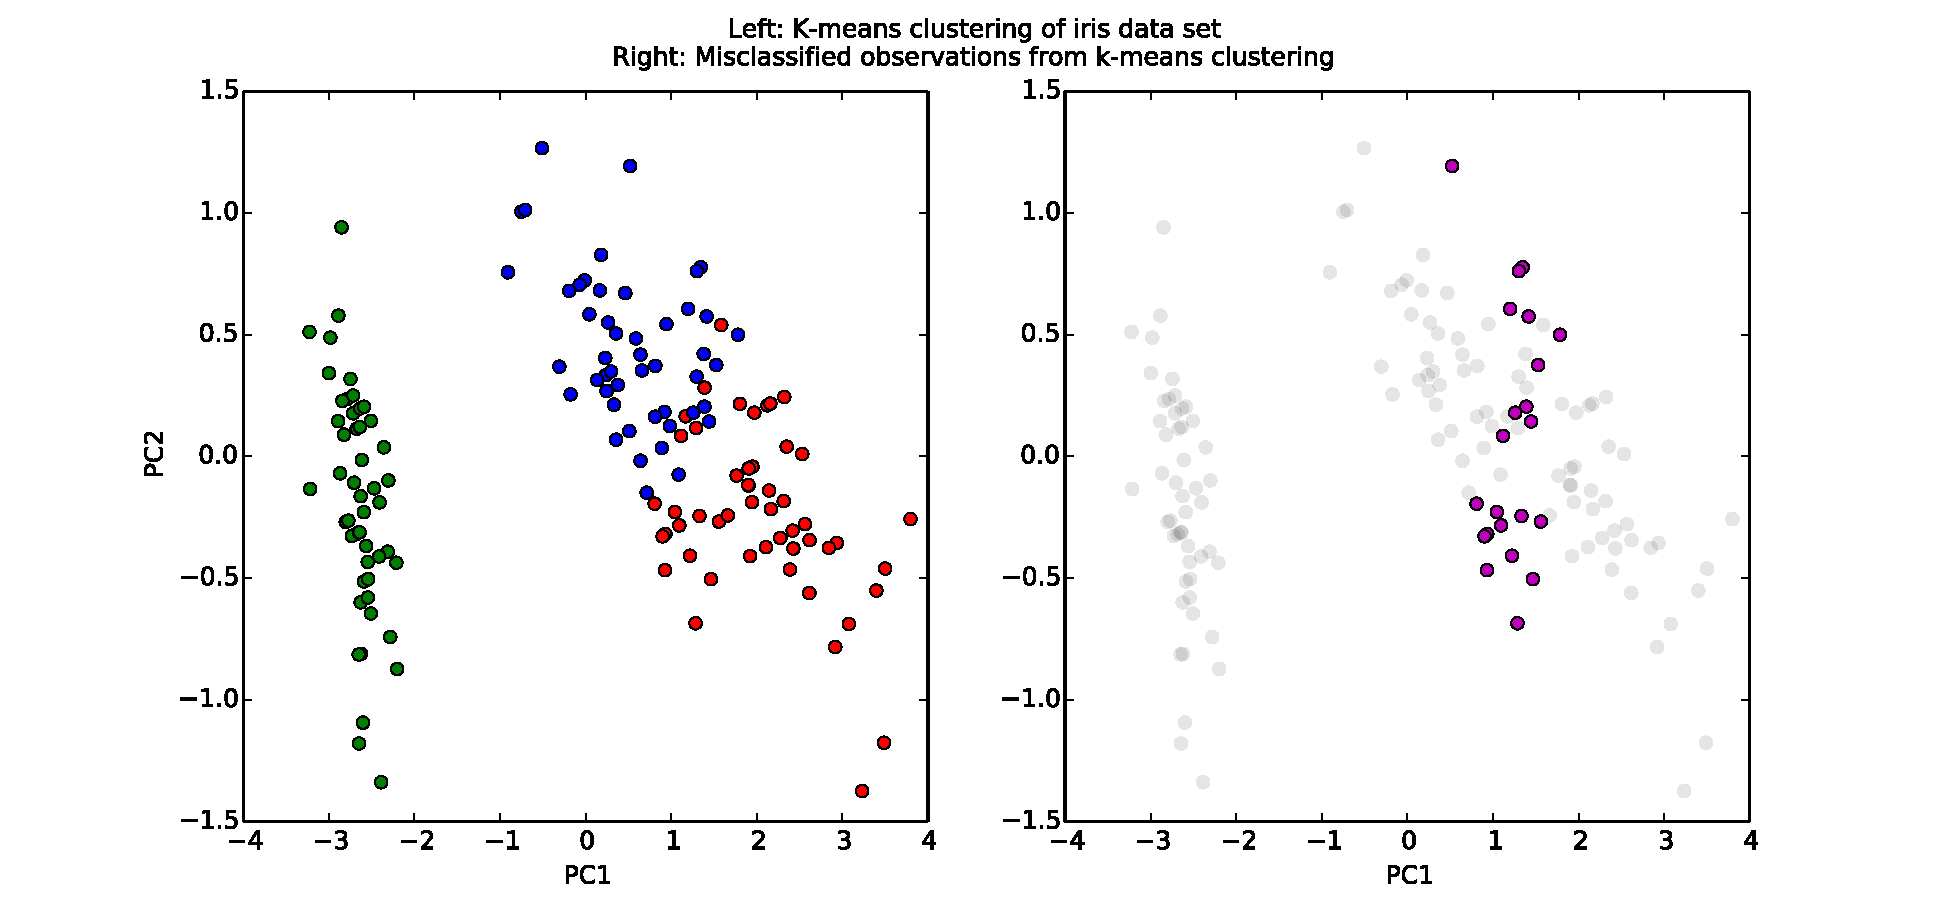
\includegraphics[width=0.9\textwidth]{./fig-python-kmeans.pdf}
  \caption{Results of applying k-means clustering to the iris data set, using the k-means algorithm impelmented in SciPy.\label{fig:pykmeans}}
\end{figure}


\section{Gaussian Mixture Models in R}

There are multiple packages for fitting mixture models in R.  We'll look at two -- |mixtools| and |MCLUST|.

\subsection{Installing mixtools}

The package |mixtools| can be installed via the GUI or the |install.packages| command. A \href{http://cran.r-project.org/web/packages/mixtools/vignettes/vignette.pdf}{mixtools vignette} can be downloaded from the CRAN website.

\subsection{Using mixtools}

We'll look at how to use mixtools using a data set on eruption times for the Old Faithful geyser in Yellowstone National Park (|?faithful| for details). We'll fit a univariate Gaussian mixture model to the time between eruptions data (\verb|faithful$waiting|).

\begin{R}
# allows us to refer to the variables within waiting time
# without using the standard list "$" syntax
> attach(faithful)

# create a nice histogram
> hist(waiting, main = "Time between Old Faithful eruptions",
xlab = "Minutes", ylab = "", cex.main = 1.5, cex.lab = 1.5, cex.axis = 1.4)

> library(mixtools)
> ?normalmixEM  # read the docs!
> wait.mix <- normalmixEM(waiting)

> names(wait.mix)
[1] "x"          "lambda"     "mu"         "sigma"      "loglik"     "posterior"
[7] "all.loglik" "restarts"   "ft"

# lambda is what we called "pi" in the lecture notes
> wait.mix[c("lambda","mu","sigma")]

> class(wait.mix)
[1] "mixEM"
> ?plot.mixEM  # read about the plotting options for the mixEM object
> plot(wait.mix, density=TRUE)
> plot(wait.mix, loglik=FALSE, density = TRUE, cex.axis = 1.4, cex.lab = 1.4, cex.main = 1.8, main2 = "Time between Old Faithful eruptions", xlab2 = "Minutes")
\end{R}%$


\begin{figure}[!ht]
    \centering
    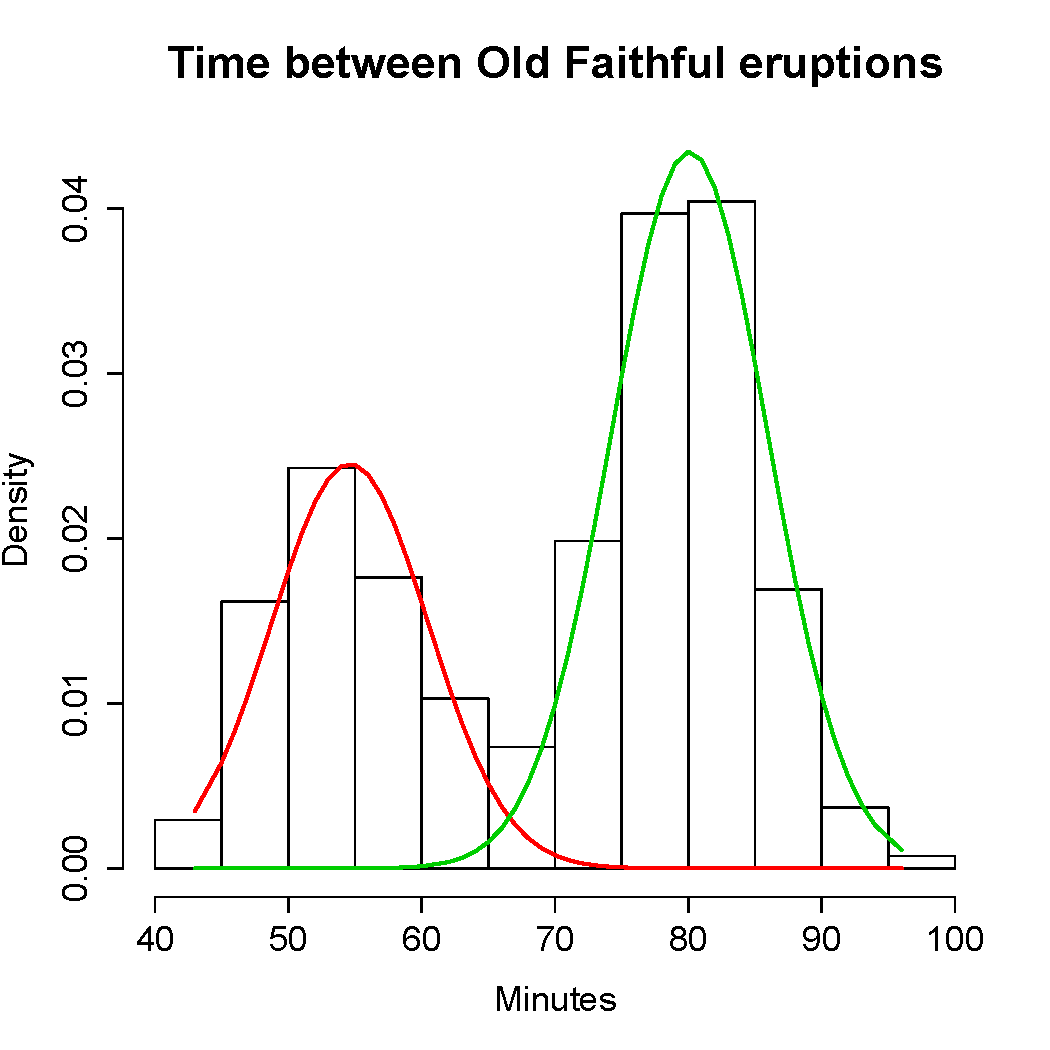
\includegraphics[width=0.5\columnwidth]{./faithful-R.pdf}
    \caption{A Gaussian mixture model for the Old Faithful dataset, estimated using the mixtools module in R.}\label{fig:faithfulR}
\end{figure}


\subsection{Installing MCLUST}
The package |MCLUST| is one of another package that provides maximum likelihood based estimation of mixture models.  You will need to install the package (and it's dependencies) from the R GUI or using the |install.packages| command (|install.packages("mclust", dependencies=T)|).

\subsection{Using MCLUST}

We're going to use two data set to illustrate some of |MCLUST|'s capabilities -- the iris data set we've worked with before, and the bivariate version of the Old Faithful data set. We'll start off with  the old faithful data set.

\begin{R}
> plot(faithful$eruptions, faithful$waiting)
\end{R}

From visual inspection of the bivariate scatter plot, it looks like there two clusters. Let's apply the |Mclust| function and see what it suggests:

\begin{R}
> library(mclust)
> fclust <- Mclust(faithful)
> fclust

 best model: elliposidal, equal variance with 3 components
\end{R}

Now that we've running the mixture model, let's look at the results graphically. The following call to |plot| will produce a series of plots.

\begin{R}
> plot(fclust)
\end{R}

The first plot gives is a diagnostic plot that shows the likelihood of the model as a function of  the number of groups (see BIC below). In general, when considering many possible models you want to pick the simplest model that has a highest likelihood. The second graphically represents the classification. The third plots highlights those objects for which the cluster assignment is most uncertain. The fourth plot gives a graphical representation of the Gaussian densities.

The |Mclust| function used a likelihood criterion called the ``Bayesian Information Criterion'' (BIC) to estimate the number of components (clusters) in the mixture model. By this criterion it suggested 3 components. BIC, like other information criteria (the Akaike Information Criterion is another popular one), is designed to help choose among parametric models with different numbers of parameters. It tries to choose the simplest model that provides a good fit to the data.

\begin{R}
> names(fclust)
 [1] "modelName"      "n"              "d"              "G"              "BIC"
 [6] "bic"            "loglik"         "parameters"     "z"              "classification"
[11] "uncertainty"
> ?mclust  # check out the docs to read about all the returned parameters
\end{R}

Of course you don't have to accept the number of clusters that the |Mclust| function estimated. Here's how you'd calculate the mixture model with a user determined number of clusters:

\begin{R}
> fclust2 <- Mclust(faithful, G=2)
> plot(fclust2)
\end{R}

% Now let's generate some diagnostic plots for the mixture model:

% \begin{R}
% > plot(fclust)
% \end{R}

If you wanted to generate some of those plots individually you can do the following:

\begin{R}
# generate a plot showing the classifications predicted by mixture model
> mclust2Dplot(data = faithful, what = "classification", identify = TRUE,
    parameters = fclust$parameters, z = fclust$z)
\end{R}

See the docs for the |mclust2Dplot| function for other options.

\subsection{Mixture Models for the Iris data set}

The |MCLUST| package includes the function |clPairs|, a very nice extension of the |pairs| function, for creating scatter plot matrices with group information. The following code illustrates this:

\begin{R}
> names(iris) # remind yourself of the variables in the iris data set
[1] "Sepal.Length" "Sepal.Width"  "Petal.Length" "Petal.Width"  "Species"

# 5th variable is the Species classification
> clPairs(data=iris[,-5], classification=iris[,5])
\end{R}

\begin{figure}[!ht]
    \centering
    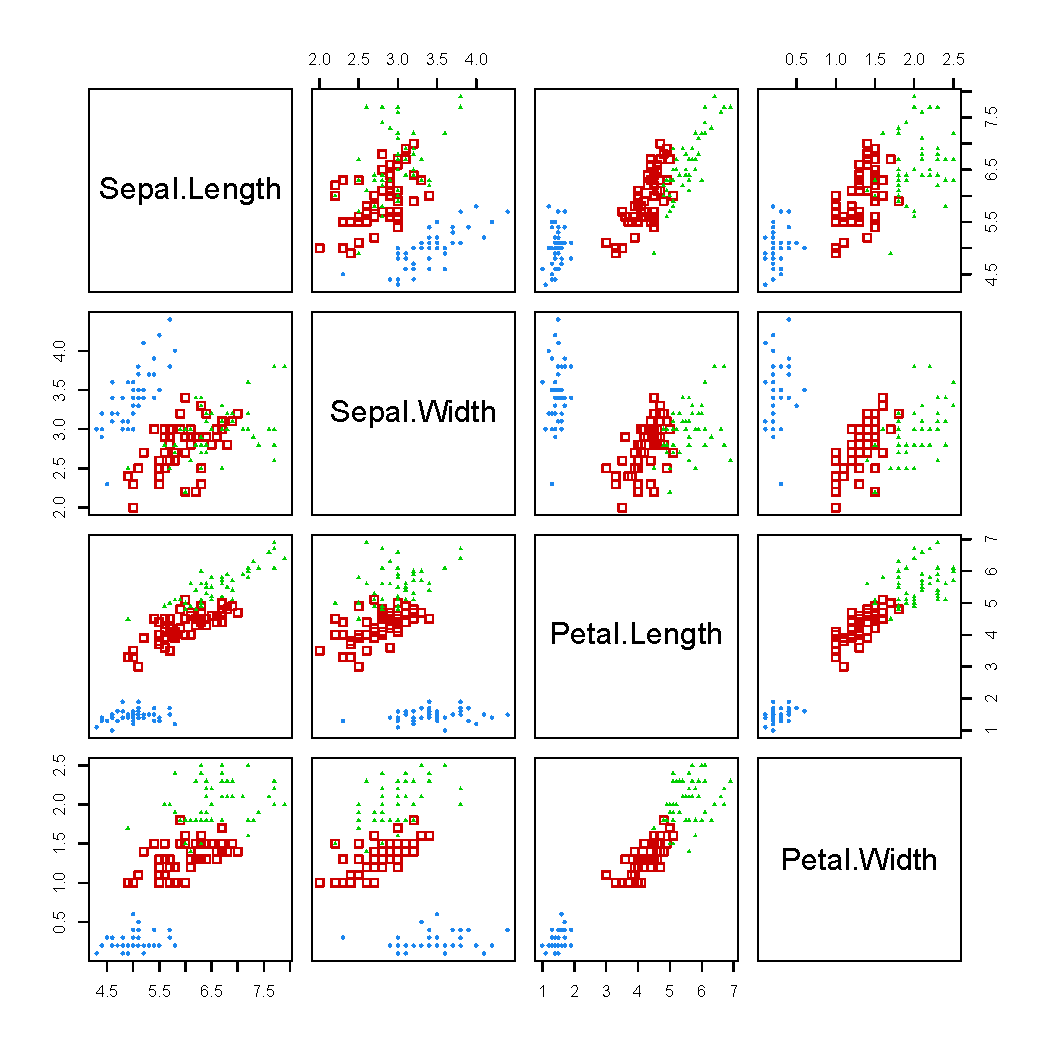
\includegraphics[width=0.5\columnwidth]{./iris-clpairs.pdf}
    \caption{Output of the \texttt{clpairs} function for the iris data set.}\label{fig:clpairs}
\end{figure}

Let's see what |Mclust| makes of the iris data set:
%
\begin{R}
> iclust <- Mclust(iris[,-5])
> iclust

 best model: ellipsoidal, equal shape with 2 components
> plot(iclust)
\end{R}
%
Blind to the actual group structure the BIC suggests just two components, whereas we know there are three groups (though \textit{I. versicolor} is thought to be an allopolyploid hybrid; see Kim et al. (2007) Ann Bot, 100: 219-224). Examine the first graph produced by the |plot| call above to see how the 2 and 3 component models compare with respect to the BIC.

Now let's see how the mixture model does when we give it the true number of clusters:
%
\begin{R}
> iclust3 <- Mclust(iris[,-5], G=3)
> plot(iclust3)
\end{R}

To calculate the classification error rate we can compare the estimated clustering to the "true" (known) classification with the |classError| function (|?classError| for details):
%
\begin{R}
> classError(iclust3$classification, iris[,5])
$misclassified
[1] 69 71 73 78 84

$errorRate
[1] 0.03333333
\end{R}

The |uncerPlot| command allows us to visualize the uncertainty implied by the mixture model to see how uncertain the model was about the misclassified samples.
%
\begin{R}
> uncerPlot(iclust3$z, iris[,5])
\end{R}
%
In the uncertainty plot the vertical lines indicate the misclassified samples. As you can see those tend to be among the observations that the mixture model was most uncertain about with respect to which component they belonged to.


\subsection{More details on MCLUST}

See the \href{http://www.stat.washington.edu/research/reports/2006/tr504.pdf}{MCLUST docs} for in depth discussion of the use of |MCLUST|. The examples illustrated above were drawn from this documentation.


\section{Mixture Modeling in Python}

The package \href{http://scikit-learn.org/stable/}{scikit-learn} extends the SciPy library with a number of common machine learning algorithms, including an implementation of Gaussian mixture modeling.  |scikit-learn| is included with the Anaconda Python distribution you have already installed. The code below demonstrates how to use |scikit-learn| to carry out mixture modeling.

Before you get started use the the |write.table()| function in R to create a tab-delimited version of the |faithful| dataset (hint: use |"\t"| to specify tabs as the separator character, and dont include row names in the file). If you've properly formatted the file you should be able to open it as follows, and create a histogram:
%
\begin{python}
In [1]: faithful = pd.read_table('/home/pmagwene/faithful.txt')
In [2]: f = faithful.values
In [3]: f.shape
Out[3]: (272, 2)
\end{python}
%
Assuming that worked, let's import |scikit-learn| and fit a mixture model:
%
\begin{python}
In [4]: from sklearn import mixture
In [6]: classifier = mixture.GMM(n_components = 2)
In [7]: fit = classifier.fit(f[:,1])

In [22]: fit.means_  # means of the estimated subdistributions
Out[22]:
array([[ 80.12056513],
       [ 54.6623402 ]])

In [23]: fit.covars_  # (co)variances of the estimated substrituions
Out[23]:
array([[ 34.08969904],
       [ 34.95662279]])

In [66]: fit.weights_   #  weighting factors (pi in slides)
Out[66]: array([ 0.63770034,  0.36229966])

In [32]: x = np.linspace(40, 100, 200) # points at which to evaluate the model

# plot histogram using prob density rather than straight up frequency
In [33]: hist(f[:,1], normed=True, alpha=0.2, color='gray')

# draw the PDFs for the two estimated subdistributions
# notice how we multiply each normal PDF by it's weight

In [63]: plot(x, fit.weights_[0] * normpdf(x, fit.means_[0], sqrt(fit.covars_[0])),color='red')
In [64]: plot(x, fit.weights_[1] * normpdf(x, fit.means_[1], sqrt(fit.covars_[1])),color='blue')
In [73]: xlabel("Waiting Time")
In [74]: ylabel("Density")
In [75]: title("Time between Old Faithful eruptions")
\end{python}

\begin{figure}[!ht]
    \centering
    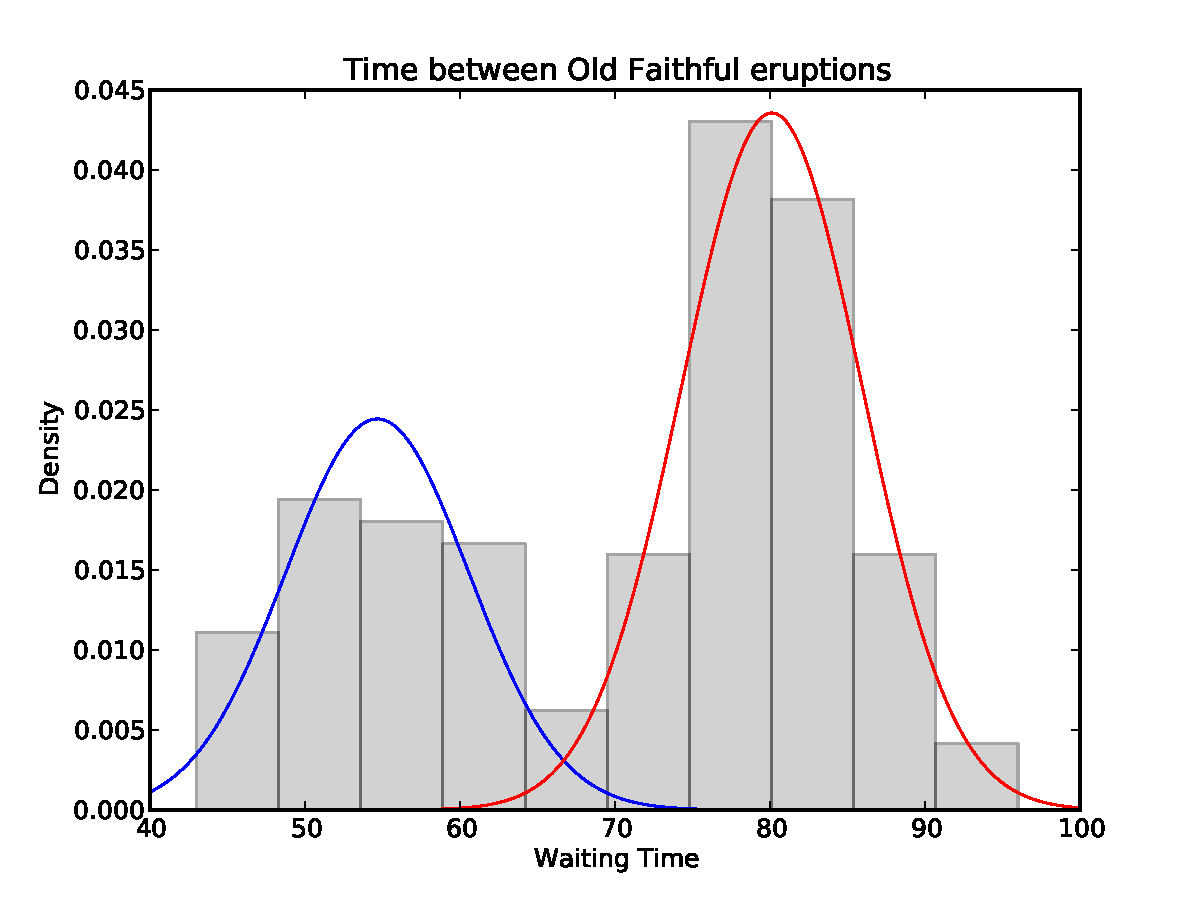
\includegraphics[width=0.5\columnwidth]{./faithful-python.pdf}
    \caption{A Gaussian mixture model for the waiting time variable in the Old Faithful dataset, estimated using the scikit-learn module in Python.}\label{fig:faithfulpy}
\end{figure}

Now let's look at the binary data:
%
\begin{python}
In [4]: plot(f[:,0], f[:,1], 'k.')  # 'k.' gives small black dots as plot points
In [8]: xlabel("Eruption time (mins)")
In [9]: ylabel("Waiting time to next eruption (mins)")

# specify covariance_type = 'full' to estimate complete covariance matrices
In [10]: classifier2 = mixture.GMM(n_components=2, covariance_type='full')
In [11]: fit2 = classifier2.fit(f)

# setup grid to evaluate mixture model over
In [12]: x = linspace(1.5,5,200)
In [13]: y = linspace(40,100,100)
In [14]: X,Y = meshgrid(x, y)
In [23]: XY = np.c_[X.ravel(), Y.ravel()] # like R's c()

# evaluate the mixture model over the grid
In [24]: Z = log(-fit2.eval(XY)[0])
In [25]: Z = Z.reshape(X.shape)
In [26]: cntr = contour(X, Y, Z)
\end{python}
Check out the |scikit-learn| docs for more details and examples.

\begin{figure}[!ht]
    \centering
    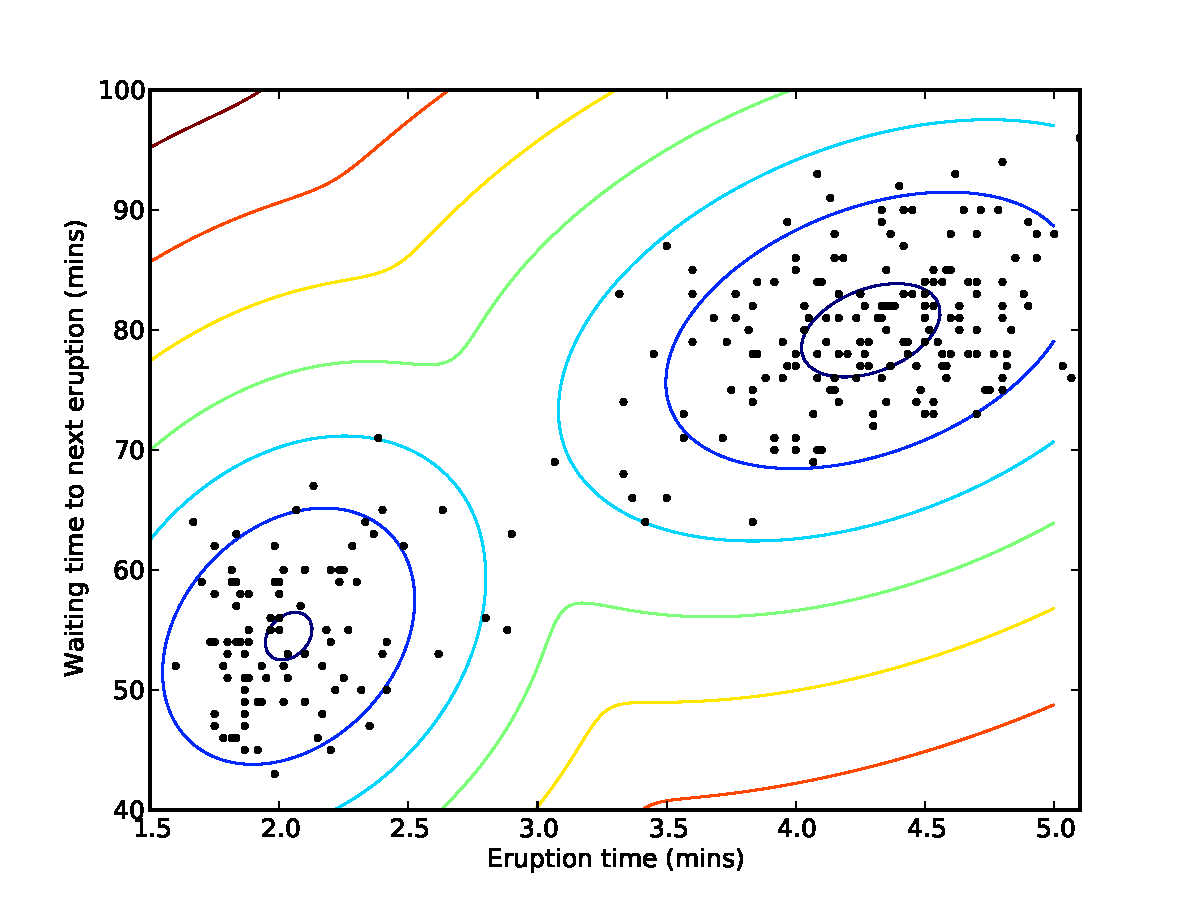
\includegraphics[width=0.5\columnwidth]{./faithful2d-python.pdf}
    \caption{A Gaussian mixture model for 2D Old Faithful dataset, estimated using the scikit-learn module in Python.}\label{fig:faithfulpy2}
\end{figure}


\begin{assignment}
Download the dataset |ddata.txt| from the course wiki. This data set consists of 64 variables measured on 720 specimens. Use the various clustering and ordination techniques you've learned over the course of the semester to explore this data set and estimate the number of clusters in the data.  Use code and figures to support your conclusion.  Hint: you might consider using a lower dimensional approximation of the data to facilitate your analyses.

\smallskip
You're free to use either R or Python.  If using Python, submit your assignment as an IPython notebook; when using R submit your assignment as a knitr document.

\end{assignment}


\section{Multidimensional Scaling in R}

\subsection{Metric MDS}

The implementation of classic metric scaling in R is carried out using the |cmdscale()| function. Read the documentation for |cmdscale| and then work through the example showing the application of MDS to analysis of road distances between US cities available at the following link (but see notes below first):

\href{http://personality-project.org/r/mds.html}{http://personality-project.org/r/mds.html}.

\medskip
As you work through your example note the following:

\begin{itemize}
\item You can use the |source()| function not only with a local file but also with a URL.  This is convenient but potentially a security issue so don't run code willy nilly without checking out what it does.

\item You can download the code at \href{http://personality-project.org/r/useful.r}{http://personality-project.org/r/useful.r} and check out the functions that it includes. I thought the |read.clipboard()| function was particularly nice.
\end{itemize}



% \subsection{Non-metric MDS}

% The |isoMDS()| function in the |MASS| package implements the Shepard-Kruskal version of non-metric scaling, while the |sammon()| function in the same package use the criterion proposed by Sammon (1969). You will need to utilize these functions, along with |cmdscale| and the hierarchical clustering functions covered last week for the following assignment.



\section{Multidimensional Scaling in Python}

The scikit-learn package also includes facilities for metric and non-metric multidimensional scaling.  The functions for carrying out MDS are included in the |sklearn.manifold| module which also includes a variety of other techniques for so-called `manifold learning'.  Manifold learning is an area of the machine learning literature concerned with approaches to non-linear dimensionality reduction.

We'll apply metric MDS to the iris data set, using Euclidean distance as our dissimilarity measure.  Recall that metric MDS on Euclidean distances is equivalent to PCA.
%
\begin{python}
>>> import sklearn.datasets
>>> iris = sklearn.datasets.load_iris()
>>> print iris['DESCR']
Iris Plants Database

Notes
-----
Data Set Characteristics:
    :Number of Instances: 150 (50 in each of three classes)
    :Number of Attributes: 4 numeric, predictive attributes and the class
    :Attribute Information:
        - sepal length in cm
... Output Truncated ...

>>> iris.data
array([[ 5.1,  3.5,  1.4,  0.2],
       [ 4.9,  3. ,  1.4,  0.2],
       [ 4.7,  3.2,  1.3,  0.2],
       [ 4.6,  3.1,  1.5,  0.2],
... Output Truncated ...

>>> import sklearn.manifold

# we setup the model first, asking for a two dimensional embedding (n_components)
>>> mds = sklearn.manifold.MDS(dissimilarity='euclidean', n_components=2)  
>>> pos = mds.fit_transform(iris.data)  # and then we fit the model to the data

# fti_transforms returns an array that
# holds the information about coordinates in the MDS space
>>> pos.shape
(150, 2)

# plot the ordination
>>> plot(pos[:,0], pos[:,1], 'ko')
[<matplotlib.lines.Line2D object at 0x10d683b50>]
>>> gca().set_aspect('equal')
>>> draw()
\end{python}

% \subsection{Non-metric MDS in scikit-learn}
% Non-metric MDS in sklearn uses an approach entitled ``SMACOF (Scaling by Majorizing a Complicated Function) '' (see Borg I, Groenen PJF (2005). Modern Multidimensional Scaling: Theory and Applications. 2nd edition. Springer, New York.).  The non-metric MDS call is a simple modification of the MDS:
% %
% \begin{python}
% >>> nmds = sklearn.manifold.MDS(metric=False, dissimilarity='euclidean')
% >>> nmds.fit(iris.data)
% MDS(dissimilarity='euclidean', eps=0.001, max_iter=300, metric=False,
%   n_components=2, n_init=4, n_jobs=1, random_state=None, verbose=0)
% >>> plot(nmds.embedding_[:,0], nmds.embedding_[:,1], 'ko')
% [<matplotlib.lines.Line2D object at 0x10bec9450>]
% >>> gca().set_aspect('equal')
% >>> draw()
% \end{python}


% \subsection{Comparing the Metric and Non-Metric MDS in Python}
The iris data set, as represented in sklearn, has a variety of accessory attributes.  For example, the |target_names| attribute gives the set of species labels, and the 'target' attribute gives the corresponding classification for each sample.  We will use this to create a fancier MDS ordination plot.
%
\begin{python}
>>> iris.target_names
array(['setosa', 'versicolor', 'virginica'], 
      dtype='|S10')
>>> iris.tar
iris.target        iris.target_names  
>>> iris.target
array([0, 0, 0, 0, 0, 0, 0, 0, 0, 0, 0, 0, 0, 0, 0, 0, 0, 0, 0, 0, 0, 0, 0,
       0, 0, 0, 0, 0, 0, 0, 0, 0, 0, 0, 0, 0, 0, 0, 0, 0, 0, 0, 0, 0, 0, 0,
       0, 0, 0, 0, 1, 1, 1, 1, 1, 1, 1, 1, 1, 1, 1, 1, 1, 1, 1, 1, 1, 1, 1,
       1, 1, 1, 1, 1, 1, 1, 1, 1, 1, 1, 1, 1, 1, 1, 1, 1, 1, 1, 1, 1, 1, 1,
       1, 1, 1, 1, 1, 1, 1, 1, 2, 2, 2, 2, 2, 2, 2, 2, 2, 2, 2, 2, 2, 2, 2,
       2, 2, 2, 2, 2, 2, 2, 2, 2, 2, 2, 2, 2, 2, 2, 2, 2, 2, 2, 2, 2, 2, 2,
       2, 2, 2, 2, 2, 2, 2, 2, 2, 2, 2, 2])

# setup Boolean vectors to represent the different species
>>> setosa = iris.target == 0
>>> versicolor = iris.target == 1
>>> virginica = iris.target == 2
>>> plot(pos[setosa,0], pos[setosa,1], 'ro', label='I. setosa')
>>> plot(pos[versicolor,0], pos[versicolor,1], 'g*', label='I. versicolor')
>>> plot(pos[virginica,0], pos[virginica,1], 'b^', label='I. virginica')
>>> gca().set_aspect('equal')
\end{python}

%%% Local Variables:
%%% TeX-master: "handout-clustering2.tex"
%%% End: